% Drawing a graph
% Author: Stefan Kottwitz
% https://www.packtpub.com/hardware-and-creative/latex-cookbook
\documentclass[border=10pt]{standalone}
%\usepackage{tkz-graph}
\usepackage{tikz}
\usetikzlibrary{positioning}
%\usepackage{mathpazo}
\newcounter{row}
\newcounter{col}

%\GraphInit[vstyle = Shade]
%\tikzset{
%  LabelStyle/.style = { rectangle, rounded corners, draw,
%                        minimum width = 2em,
%                        text = black, font = \bfseries },
%  VertexStyle/.append style = { inner sep=5pt,
%                                font = \Large\bfseries},
%  EdgeStyle/.append style = {->, bend left} }
%\thispagestyle{empty}
\begin{document}


\newcommand\setrow[5]{
\setcounter{col}{1}
\foreach \n in {#1, #2, #3, #4, #5} {

	\edef\x{\value{col} - 0.5}
	\edef\y{5.5 - \value{row}}
	\node[anchor=center] at (\x, \y) {\n};
	\stepcounter{col}
	}
	\stepcounter{row}
}



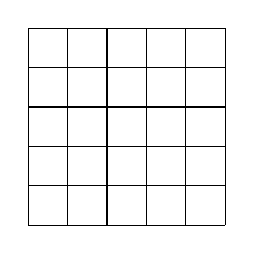
\begin{tikzpicture}[scale=0.5]
\begin{scope}[font=\sffamily\slshape]
\draw (0,0) grid (5,5);
%\draw[thick, scale=3] (0,0) grid (3, 3);

\setcounter{row}{1}
\setrow {25}{24}{22}{19}{15}
\setrow {23}{21}{18}{14}{10}
\setrow {20}{17}{13}{9}{6}
\setrow {16}{12}{8}{5}{3}
\setrow {11}{7}{4}{2}{1}

%\setrow {1}{2}{3}{4}{5}{6}{ }{ }{ }{}
%\setrow {2}{ }{ } {4}{ }{ } { }{ }{ }{}
%\setrow {}{}{3} {}{}{} {}{}{}{}
%\setrow {}{}{} {}{}{} {}{}{}{}
%\setrow {}{}{} {}{}{} {}{}{}{}
%\setrow {}{}{} {}{}{} {}{}{}{}
%\setrow {}{a}{} {c}{}{} {}{}{}{}
%\setrow {}{}{} {}{}{} {}{}{}{}
%\setrow {}{}{} {}{}{} {}{}{}{}
%\setrow {}{}{} {}{}{} {}{}{}{}
%\node[anchor=center] at (4.5, -0.5) {1};

\end{scope}


\end{tikzpicture}


\end{document}

